\section{Question 5}
% 
% 
\subsection{Vector Length and Angle Calculation}
% 
% 
\begin{lstlisting}[style=pystyle]
import numpy as np

# Define the vectors u and v
u = np.array([5, 6])
v = np.array([1, -2])

# Calculate the length of vector u
length_u = np.linalg.norm(u)

# Calculate the length of vector v
length_v = np.linalg.norm(v)

# Calculate the dot product of u and v
dot_product_uv = np.dot(u, v)

# Calculate the angle between u and v (in radians)
cosine_theta = dot_product_uv / (length_u * length_v)
theta = np.arccos(cosine_theta)

# Convert the angle from radians to degrees
theta_degrees = np.degrees(theta)

# Print the results
print("Length of u:", length_u)
print("Length of v:", length_v)
print("Angle between u and v (in radians):", theta)
print("Angle between u and v (in degrees):", theta_degrees)
    
\end{lstlisting}
% 
% 
\paragraph{\textbf{The output is:}}
\begin{itemize}
    \item Length of u: 7.810249675906654
    \item Length of v: 2.23606797749979
    \item Angle between u and v (in radians): 1.983206768392284
    \item Angle between u and v (in degrees): 113.62937773065683
\end{itemize}
% 
% 
% 
% 
% 
% 
\newpage
\subsection{Orthogonal Projection and Vector Visualization}
% 
% 
\begin{lstlisting}[style=pystyle]
import numpy as np
import matplotlib.pyplot as plt

# Define vectors ~u and ~v
u = np.array([5, 6])
v = np.array([1, -2])

# Calculate Proj_v(u)
proj_v_u = (np.dot(u, v) / np.dot(v, v)) * v

# Create a plot to visualize the vectors
plt.figure(figsize=(6, 6))
plt.quiver(0, 0, u[0], u[1], angles='xy', scale_units='xy', scale=1, color='b', label='Vec U')
plt.quiver(0, 0, v[0], v[1], angles='xy', scale_units='xy', scale=1, color='r', label='Vec V')
plt.quiver(0, 0, proj_v_u[0], proj_v_u[1], angles='xy', scale_units='xy', scale=1, color='g', label='Proj_v(u)')

# Set plot limits
plt.xlim(-4, 8)
plt.ylim(-4, 8)

# Add labels and legend
plt.xlabel('X')
plt.ylabel('Y')
plt.legend()

# Show the plot
plt.grid(True)
plt.show()

\end{lstlisting}



% Orthogonal_Projection
\begin{figure}[H]
    \centering
    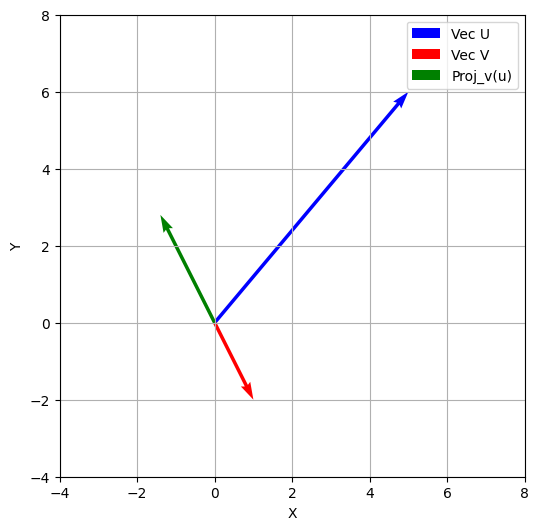
\includegraphics[width=0.75\textwidth]{pic/Orthogonal_Projection.png}
    \caption{Orthogonal Projection of the Vector $\vec{u}$ onto $\vec{v}$}
\end{figure}